% =====================================================================
\lecture{6}{אינפלציה}{מפגש 3, שעה וחצי. \ (20' הבעיות, 25' שדה סקלרי ו-\en{slow roll}, 25' הפרעות, 20' תחזיות ותרגילים)}
% =====================================================================

\begin{goalbox}
\textbf{מטרות.} (1) לנסח את בעיות האופק, השטיחות והשרידים. (2) להראות שתקופה של רדיוס האבל נע מתכווץ פותרת את כולן. (3) לממש אותה בשדה סקלרי בגלגול איטי. (4) לגזור את ספקטרום ההפרעות ואת $n_s$ ו-$r$, ולהשוות לתצפית.
\end{goalbox}

\subsection{שלוש בעיות במפץ הגדול החם}
\textbf{אופק.} ב-\en{EdS} האופק בזמן הפיזור האחרון נראה היום בזווית $\theta_H\approx\chi_{\rm p}(z_\star)/D_M(z_\star)\approx\sqrt{1/(1+z_\star)}\approx1.7^\circ$ (ב-$\LCDM$ קרוב ל-$1^\circ$). בשמיים יש $\sim10^4$ אזורים שלא היו בקשר סיבתי, ובכל זאת $T$ זהה עד $10^{-5}$.

\textbf{שטיחות.} מפרידמן:
\begin{equation}
|\Omega-1|=\frac{|k|c^2}{(aH)^2}\propto\begin{cases}a^2&\text{קרינה}\\ a&\text{חומר}\end{cases}
\end{equation}
כלומר שטיחות היא נקודת שיווי משקל \emph{לא יציבה}. היום $|\Omega_k|\lesssim0.002$, ולכן ב-\en{BBN} $|\Omega-1|\lesssim10^{-18}$ ובזמן פלאנק $\lesssim10^{-62}$ (תרגיל 6.1).

\textbf{שרידים.} תיאוריות איחוד מייצרות מונופולים מגנטיים ב-$T\sim10^{16}\,\mathrm{GeV}$; בכמות שהיו סוגרים את היקום פי $10^{11}$. לא נצפו.

\subsection{הפתרון: רדיוס האבל נע מתכווץ}
כל שלוש הבעיות נובעות מכך ש-$(aH)^{-1}$ (רדיוס האבל הנע) \emph{גדל} תמיד בקרינה ובחומר. אם בעבר הוא \emph{קטן}:
\begin{equation}
\frac{d}{dt}\Big(\frac{1}{aH}\Big)<0\iff\ddot a>0\iff w<-\tfrac13 .
\end{equation}
\begin{itemize}
\item אופק: אזור קטן בקשר סיבתי מתנפח לגודל של כל היקום הנצפה.
\item שטיחות: $|\Omega-1|\propto(aH)^{-2}$ קטן במהירות; אחרי $N$ \en{e-folds} בפקטור $e^{-2N}$.
\item שרידים: מדוללים בפקטור $e^{-3N}$.
\end{itemize}
מספיק $N\gtrsim50$--$60$ \en{e-folds} ($a\to e^{60}a$), תלוי בסולם האנרגיה ובחימום מחדש.

\subsection{שדה סקלרי}
לשדה הומוגני $\phi(t)$ בפוטנציאל $V(\phi)$ (יחידות $\hbar=c=1$, $M_{\rm Pl}^{-2}=8\pi G$):
\begin{equation}
\rho=\tfrac12\dot\phi^2+V,\qquad p=\tfrac12\dot\phi^2-V,\qquad
\ddot\phi+3H\dot\phi+V'(\phi)=0,\qquad H^2=\frac{1}{3M_{\rm Pl}^2}\Big(\tfrac12\dot\phi^2+V\Big).
\end{equation}
אם $\dot\phi^2\ll V$ אז $w\approx-1$: אינפלציה. האיבר $3H\dot\phi$ הוא חיכוך --- כדור שמתגלגל באיטיות בשמן.

\begin{keybox}
\textbf{קירוב הגלגול האיטי (\en{slow roll}).} $3H\dot\phi\simeq-V'$, \ $H^2\simeq V/3M_{\rm Pl}^2$. פרמטרים:
\begin{equation}
\epsilon_V=\frac{M_{\rm Pl}^2}{2}\Big(\frac{V'}{V}\Big)^2\ll1,\qquad
\eta_V=M_{\rm Pl}^2\frac{V''}{V},\ \ |\eta_V|\ll1,\qquad
N=\int_{\phi_{\rm end}}^{\phi_*}\frac{V}{M_{\rm Pl}^2V'}\,d\phi .
\end{equation}
האינפלציה נגמרת כש-$\epsilon_V\simeq1$. $\epsilon=-\dot H/H^2$, ולכן $\ddot a>0\iff\epsilon<1$.
\end{keybox}
\textbf{חימום מחדש.} בסוף, $\phi$ מתנודד סביב המינימום ($\langle w\rangle=0$) ודועך לחלקיקי המודל הסטנדרטי. היקום חם --- והמפץ הגדול "החם" מתחיל.

\begin{figure}[htbp]\centering
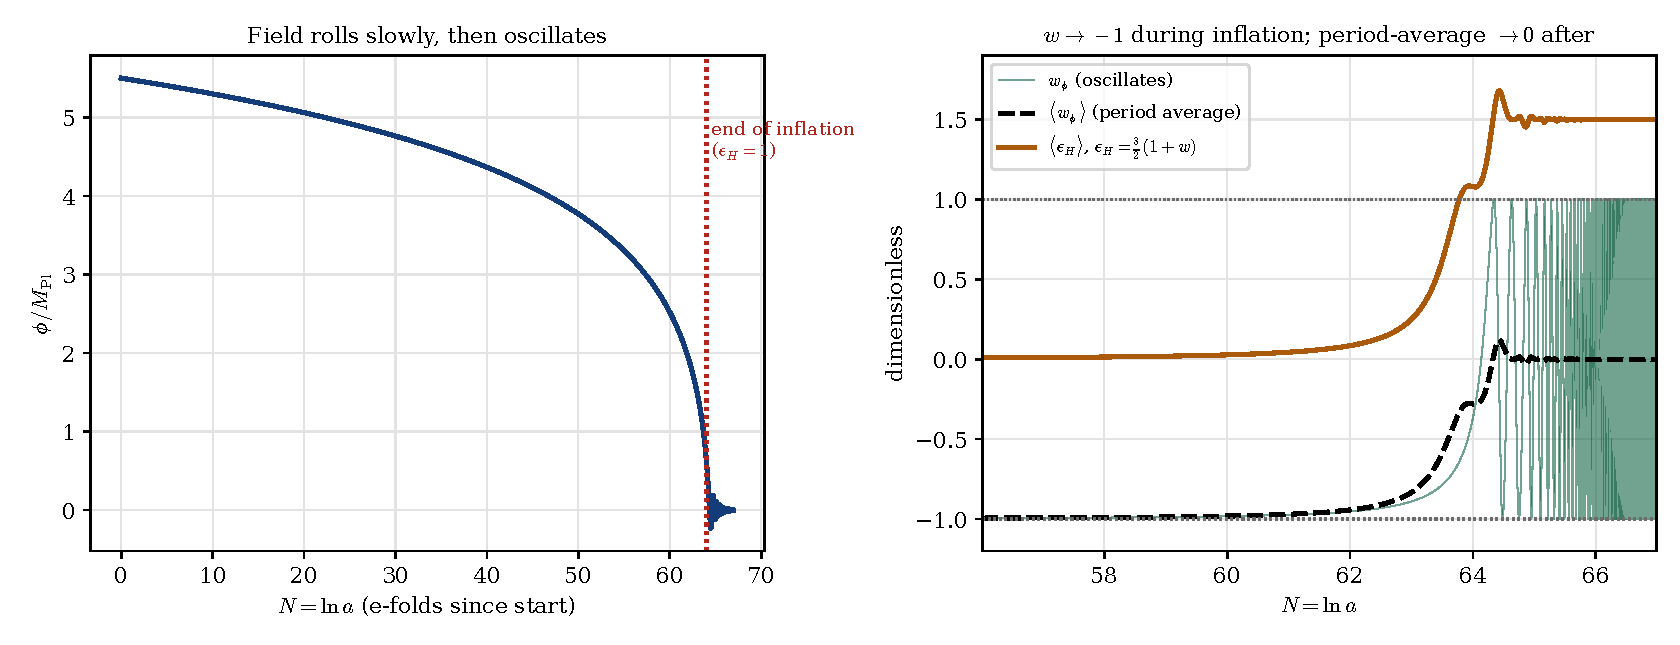
\includegraphics[width=0.9\textwidth]{figs/fig_infl_dyn.pdf}
\caption{\small דינמיקה של שדה האינפלטון: גלגול איטי, סוף האינפלציה ב-$\epsilon=1$, ותנודות.}
\end{figure}

\subsection{הפרעות}
האינפלציה לא רק מחליקה --- היא גם זורעת. תנודות קוונטיות של $\phi$ על רקע דה-סיטר:
\begin{equation}
\delta\phi\simeq\frac{H}{2\pi}\quad\text{לכל \en{e-fold}, ביציאה מהאופק }(k=aH).
\end{equation}
הן הופכות להפרעת עקמומיות $\mathcal R=-H\,\delta\phi/\dot\phi$, שנשמרת מעל האופק (הרצאה 3) עד שהמוד חוזר פנימה בעידן הקרינה וזורע את גלי הקול של הרצאה 5.
\begin{keybox}
\begin{align}
\Delta^2_{\mathcal R}(k)&=\frac{H^2}{8\pi^2\epsilon M_{\rm Pl}^2}\bigg|_{k=aH}=\frac{V}{24\pi^2\epsilon M_{\rm Pl}^4}\equiv A_s\Big(\frac{k}{k_*}\Big)^{n_s-1},
&
n_s-1&=2\eta_V-6\epsilon_V,\\
\Delta^2_t(k)&=\frac{2H^2}{\pi^2M_{\rm Pl}^2}\quad(\text{גלי כבידה}),
&
r&\equiv\frac{\Delta_t^2}{\Delta_{\mathcal R}^2}=16\epsilon_V,\quad n_t=-2\epsilon_V .
\end{align}
\end{keybox}
\textbf{היגיון ה-$n_s$:} $H$ ו-$\epsilon$ משתנים לאט במהלך האינפלציה, ולכן הספקטרום \emph{כמעט} אינווריאנטי לסולם, עם סטייה קטנה בשיעור $\epsilon,\eta\sim1/N$. ו-$r$ מודד ישירות את סולם האנרגיה: $V^{1/4}\approx1.0\times10^{16}\,\mathrm{GeV}\,(r/0.01)^{1/4}$.

\subsection{תחזיות ותצפיות}
\begin{center}\small
\begin{tabular}{@{}p{5.4cm}p{5cm}p{5.4cm}@{}}
\toprule
תחזית & מדוע & תצפית \\ \midrule
יקום שטוח & $|\Omega-1|\propto e^{-2N}$ & $\Omega_k=0.001\pm0.002$ \\
הפרעות אדיאבטיות וגאוסיות & שדה יחיד, תנודות קוונטיות ליניאריות & $f_{\rm NL}^{\rm loc}=-0.9\pm5.1$ \\
כמעט אינווריאנטי לסולם, "אדום" ($n_s<1$) & $H$ יורד לאט & $n_s=0.965\pm0.004$ (\en{Planck 2018}) \\
הפרעות מעבר לאופק ב-$z_\star$ & נוצרו באינפלציה & מתאם \en{TE} בסולמות $>1^\circ$ \\
גלי כבידה ($r$) & תנודות של המטריקה & $r<0.036$ (\en{BICEP/Keck 2021}) \\ \bottomrule
\end{tabular}
\end{center}
\textbf{מודלים.} $V=\tfrac12m^2\phi^2$: $n_s=1-2/N$, $r=8/N\approx0.13$ --- \textbf{נפסל}. \en{Starobinsky} ($R^2$): $n_s=1-2/N$, $r=12/N^2\approx0.003$ --- בלב האזור המותר. ניסויי \en{B-modes} הבאים (\en{Simons Observatory}, \en{LiteBIRD}) יגיעו ל-$r\sim10^{-3}$ ויבחנו את \en{Starobinsky} ישירות.

\begin{figure}[htbp]\centering
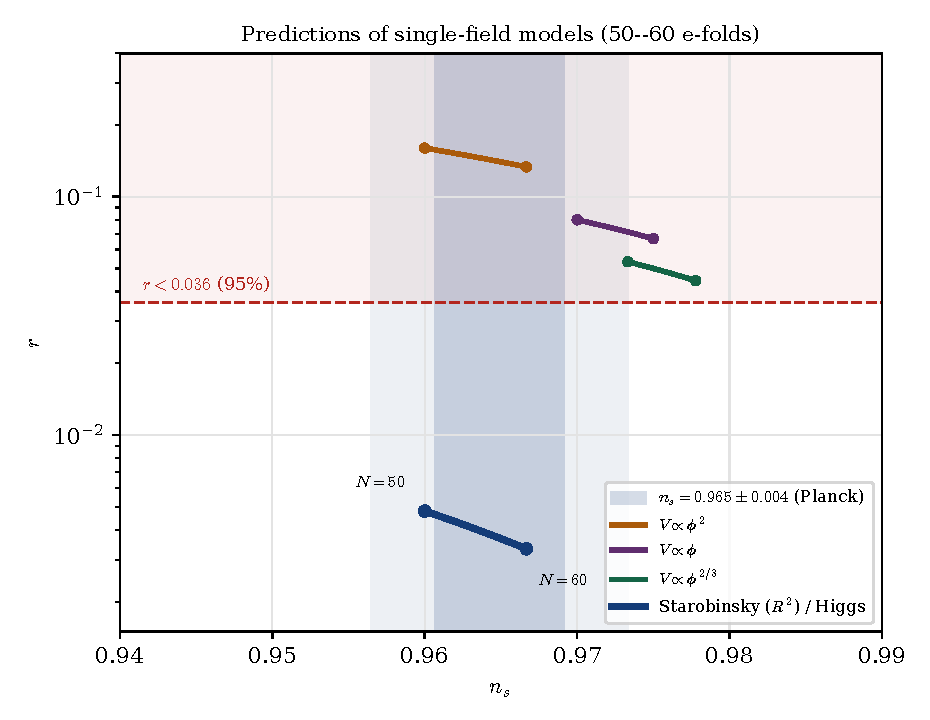
\includegraphics[width=0.6\textwidth]{figs/fig_infl_nsr.pdf}
\caption{\small המישור $(n_s,r)$: מודלים מול האזור המותר.}
\end{figure}

\begin{warnbox}
\textbf{מה אינפלציה לא פותרת.} את הקבוע הקוסמולוגי היום; את שאלת תנאי ההתחלה לאינפלציה עצמה; ואת זהות האינפלטון. היא מסגרת, לא מודל אחד.
\end{warnbox}

% ---------------------------------------------------------------------
\subsection*{תרגילים}
\begin{exercise}{כמה כוונון עדין?}
היום $|\Omega_k|<0.002$. (א) השתמשו ב-$|\Omega-1|\propto a$ (חומר) ו-$\propto a^2\propto T^{-2}$ (קרינה) כדי להעריך את $|\Omega-1|$ ב-\en{BBN} ($T=1\,\mathrm{MeV}$) ובזמן פלאנק ($T=10^{19}\,\mathrm{GeV}$); $T_{\rm eq}\approx0.8\,\mathrm{eV}$. (ב) כמה \en{e-folds} של אינפלציה מספיקים כדי ש-$|\Omega-1|=1$ לפניה ייתן את הערך מ-(א) אחריה, בסולם $T\sim10^{15}\,\mathrm{GeV}$?
\end{exercise}
\begin{solbox}
\textbf{פתרון.}\ (א) חומר: $|\Omega-1|_{\rm eq}=0.002/3400=6\times10^{-7}$. קרינה: $\times(T_{\rm eq}/T)^2$. \en{BBN}: $(0.8\,\mathrm{eV}/1\,\mathrm{MeV})^2=6.4\times10^{-13}\Rightarrow4\times10^{-19}$. פלאנק: עוד $(10^{-3}/10^{19})^2=10^{-44}\Rightarrow4\times10^{-63}$.\\
(ב) ב-$10^{15}\,\mathrm{GeV}$: $4\times10^{-19}\times(10^{-3}/10^{15})^2=4\times10^{-55}$. $e^{-2N}=4\times10^{-55}\Rightarrow N\approx63$. מכאן "60 \en{e-folds}".
\end{solbox}

\begin{exercise}{אינפלציה ריבועית, $V=\tfrac12m^2\phi^2$}
(א) חשבו $\epsilon_V$, $\eta_V$, ו-$\phi_{\rm end}$ (שבו $\epsilon_V=1$). (ב) הראו ש-$N(\phi)=(\phi^2-\phi_{\rm end}^2)/4M_{\rm Pl}^2$, ומצאו $\phi_*$ עבור $N=60$. האם השדה גדול ממסת פלאנק? (ג) חשבו $n_s$ ו-$r$. האם המודל מותר? (ד) מ-$A_s=2.1\times10^{-9}$ חשבו $m$.
\end{exercise}
\begin{solbox}
\textbf{פתרון.}\ (א) $\epsilon_V=\eta_V=2M_{\rm Pl}^2/\phi^2$; $\phi_{\rm end}=\sqrt2M_{\rm Pl}$.\\
(ב) $N=\int\frac{\phi}{2M_{\rm Pl}^2}d\phi=\frac{\phi_*^2-\phi_{\rm end}^2}{4M_{\rm Pl}^2}$; $\phi_*=\sqrt{4N+2}\,M_{\rm Pl}=15.6\,M_{\rm Pl}$: על-פלאנקי (אבל $V\ll M_{\rm Pl}^4$).\\
(ג) $n_s=1-8/(4N+2)\approx1-2/N=0.967$; $r=32/(4N+2)\approx8/N=0.13$. $n_s$ בסדר, אבל $r>0.036$: נפסל.\\
(ד) $\Delta^2_{\mathcal R}=\frac{V}{24\pi^2\epsilon_VM_{\rm Pl}^4}=\frac{m^2\phi_*^4}{96\pi^2M_{\rm Pl}^6}$ $\Rightarrow m=\sqrt{96\pi^2A_s}\,M_{\rm Pl}^3/\phi_*^2=5.8\times10^{-6}M_{\rm Pl}=1.4\times10^{13}\,\mathrm{GeV}$.
\end{solbox}

\begin{exercise}{\en{Starobinsky}}
$V=V_0\big(1-e^{-\sqrt{2/3}\,\phi/M_{\rm Pl}}\big)^2$. (א) בגבול $\phi\gg M_{\rm Pl}$, הראו $\epsilon_V\simeq\tfrac43e^{-2\sqrt{2/3}\phi/M_{\rm Pl}}$ ו-$\eta_V\simeq-\tfrac43e^{-\sqrt{2/3}\phi/M_{\rm Pl}}$. (ב) הראו $N\simeq\tfrac34e^{\sqrt{2/3}\phi/M_{\rm Pl}}$ ומכאן $n_s\simeq1-2/N$, $r\simeq12/N^2$. (ג) הציבו $N=55$ והשוו לטבלה.
\end{exercise}
\begin{solbox}
\textbf{פתרון.}\ (א) עם $\alpha=\sqrt{2/3}/M_{\rm Pl}$ ו-$e^{-\alpha\phi}\ll1$: $V'/V\simeq2\alpha e^{-\alpha\phi}$, $V''/V\simeq-2\alpha^2e^{-\alpha\phi}$. מכאן $\epsilon_V=2\alpha^2M_{\rm Pl}^2e^{-2\alpha\phi}=\tfrac43e^{-2\alpha\phi}$, $\eta_V=-\tfrac43e^{-\alpha\phi}$.\\
(ב) $N\simeq\int\frac{e^{\alpha\phi}}{2\alpha M_{\rm Pl}^2}d\phi=\tfrac34e^{\alpha\phi}$. אז $\eta_V=-1/N$, $\epsilon_V=3/4N^2$: $n_s=1+2\eta-6\epsilon\simeq1-2/N$, $r=16\epsilon=12/N^2$.\\
(ג) $N=55$: $n_s=0.964$, $r=0.004$ --- בתוך האזור המותר, ומטרה ל-\en{LiteBIRD}.
\end{solbox}
